\documentclass[UTF8]{ctexart}

\title{\huge{Swarm}}
\author{Laplx}
\date{}

\usepackage{amsmath}
\usepackage{graphicx}
\usepackage{float}
\usepackage{subfigure}

\begin{document}
	\maketitle
	\begin{abstract}
		略
	\end{abstract}
	\tableofcontents
	
	\section{数据背景与分析思路}
		\subsection{数据背景介绍}
		Swarm是一款基于位置的社交应用。用户可以使用Swarm在感兴趣的地点进行位置签到,并展示给好友。用户分为本地用户和外地(游客)用户两种。此数据集中给出了三个城市范围内的签到数据和对应签到用户的个人信息数据,分别是纽约市(nyc)、旧金山(sfo)和香港(hk)。
		
		各城市的签到数据包括8个字段:用户id,本地/外地,签到地点id,地点类型,地点类型id,地点经度、纬度,签到时间。各城市对应签到的用户数据包括6个字段:用户id,本地/外地,男/女,签到发布数,照片发布数,好友数。
		\subsection{数据加工方式与代码介绍}
		本文使用MATLAB为工具,主要加工和分析代码位于三个实时脚本(.mlx)内,分别为 describe(主要以nyc为例进行数据转换和频数统计)、analysis(对用户数据做进一步统计分析)和 difference(对hk、sfo作相似分析并合并比较)。scrap.mlx 包含一些探索性或验证性的工作并基本不出现在此文内。此外调用了五个函数 vent.m、venhd.m、idven.m、idhour.m 和 idval.m,具体说明可见函数注释。工作空间的全部变量已存储在 matlab.mat 中。
		\subsection{简要分析思路}
		本文将(按顺序)展示以下结果:
		
		\noindent 1. 签到数与地点类型、时间段的关系,并比较三座城市、当地与外地的差异。其中时间段包含小时段、星期几两个变量。\\
		2. 签到的地理分布。\\
		3. 同一用户签到的时间和空间间隔。\\
		4. 用户的签到数、照片数、好友数的分布,并进行城市和性别比较。进一步对分布做出猜想。\\
		5. 用户特征(签到数、照片数、好友数)与其签到的地点类型、时间段之间的相关性。\\
		6. 对用户及其签到特征作因子分析,给出表征性的参数。\\
		7. 聚类分析,给出各用户特征的相近程度以供参考。\\
		8. 尝试对本地用户和外地用户根据特征进行判别。
	
	\section{签到数据分析}
		\subsection{签到数与地点类型}
		首先,由于地点众多,有必要简化结构以便作进一步的初步分析。本文将签到的地点类型归为十二大类(部分类较小,部分类涵盖面较大)如下:
		
		\noindent\textbf{food}:["restaurant","bar","cafe","diner","gastropub","deli","bakeries",\\"joint","places","food"]\\
		\textbf{shop}:["mall","shop","store","market"]\\
		\textbf{work}:["office","work"]\\
		\textbf{travel}:["station","airport","bus","train","taxi","lounge","platform"]\\
		\textbf{home}:["home"]\\
		\textbf{entertain}:["neibor","event","parks","garden","theater","movie","music",\\"plaza","entertainment","club","festival"]\\
		\textbf{hotel}:["hotel","pub"]\\
		\textbf{scene}:["bridge","river","lake","road","counties","field","outdoor"]\\
		\textbf{building}:["building","cities","hall","landmark","housing","starup"]\\
		\textbf{culture}:["university","school","college","libra","galler","studio","museum",\\"art","exhi"]\\
		\textbf{sport}:["gym","stadium","play"]\\
		\textbf{life}:["bank","phar","hospital","laun","church","service","docter"]
		
		冒号后为其关键词列表,通过提取地点字段中名称是否包含该关键词进行归类。存在一定数量的地点未归入上述类别,暂不考虑这些特殊或小众的地点;注意以上类别数量总和反而超过了数据集签到条数,是由于部分地点同时带有两类关键词(具有两方面功能),应予以保留。当然,地点功能归类依靠人工设置关键词,必然存在少许偏颇、缺漏、类型不对等的情况,在后续(3.3节)中会进一步筛选和调整。
		
		随后读取 nyc\_local\_checkin.csv、nyc\_traveler\_checkin.csv、hk\_local\_\\checkin.csv、hk\_traveler\_checkin.csv、sfo\_local\_checkin.csv、sfo\_traveler\_\\checkin.csv,调用 vent 函数并进行 tabulate 统计(纵轴为频数占比),得到
		
		\begin{figure}[h]
			\centering
			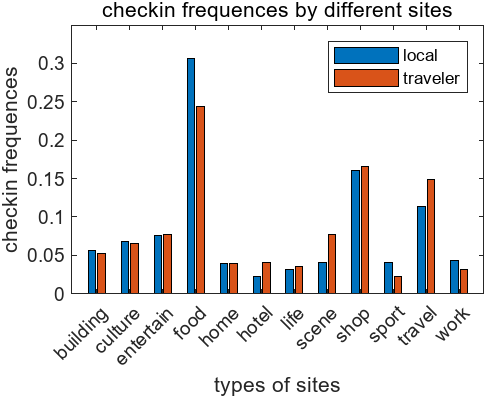
\includegraphics{checkin_sitetype_l&t.png}
			\caption{当地/外地用户签到数与地点类型分布}
			\label{ven_c_lt}
		\end{figure}
		\begin{figure}[h]
			\centering
			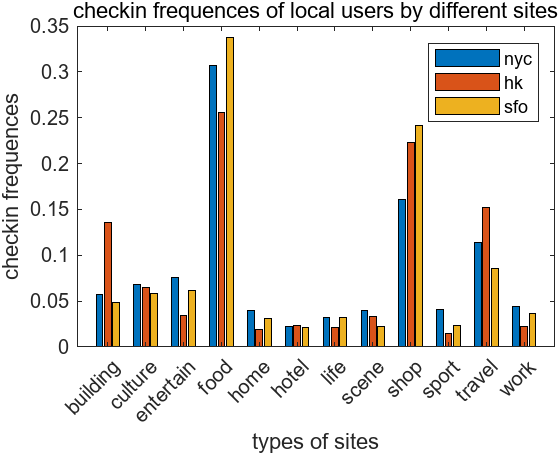
\includegraphics{checkin_sitetype_l_nhs.png}
			\caption{三城用户签到数与地点类型分布}
			\label{ven_c_nhs}
		\end{figure}
		
		图\ref{ven_c_lt} 统计了纽约市当地用户和游客用户签到地点的情况,可见 food 和 shop 为主要的两大消费目标(一是吃喝购物本身的主要性,二是这两类涵盖面也很大)。相对于当地人来说,外地游客对美食的探索并未特别熟悉,可能是停留时间较短的原因,工作、体育相关打卡也明显较少;而在宾馆、风景游览、旅途上明显多于本地人,与游客的身份相匹配,生活娱乐和购物方面也完全不输本地人。这对面向旅游业的商务提供了发展方向。
		
		图\ref{ven_c_nhs} 对比了三座城市在签到地点类型上的不同。可见香港对建筑设施、交通旅行有独特的偏好,而在自己家中、工作生活、餐饮、娱乐场所的打卡较少;旧金山在餐饮和购物两大块上非常凸出;纽约在生活、娱乐、工作、体育等个人分享色彩较浓的方面打卡比较多。国际间城市的文化和喜好差异需要受到商业关注,如旧金山的餐饮和购物可能具有更大的市场。
		
		\subsection{签到数与时间段}
		本文从具有明显周期序列特征的天和小时两个维度入手进行频数统计。天按照一星期七天进行划分,小时以四小时为一单位划分为 0-4(early morning)、4-8(morning)8-12( forenoon)、12-16(afternoon)、16-20(evening)、20-24(night)六个小时段。这里直接采用了三座城市本地人的数据进行统计,经验证外地用户的签到分布与本地几乎完全一致。
		
		图\ref{day_c_nhs} 可见香港对一周各日没有十分敏感;旧金山具有较明显的上班族的特征(周三签到数最多,周日、周一签到数最少)。
		
		图\ref{hour_c_nhs} 可见纽约夜生活比较丰富;香港在下午至晚上打卡较为普遍;旧金山同样具有明显的上班族特质(晚上和半夜打卡少,上午、傍晚打卡多)。
		
		\begin{figure}[H]
			\centering
			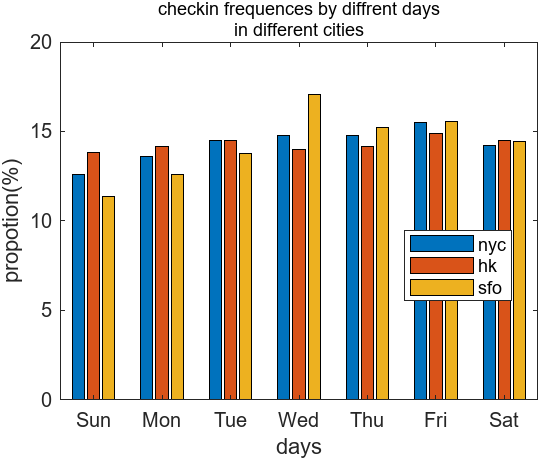
\includegraphics{checkin_day_l_nhs.png}
			\caption{三城用户签到数与一周各日分布}
			\label{day_c_nhs}
		\end{figure}
		\begin{figure}[H]
			\centering
			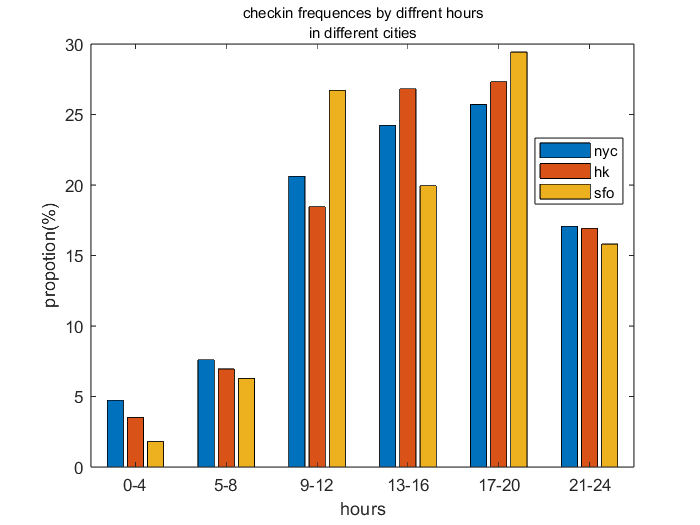
\includegraphics[scale=0.6]{checkin_hour_l_nhs.png}
			\caption{三城用户签到数与小时段分布}
			\label{hour_c_nhs}
		\end{figure}
		
		\subsection{签到地点类型与时间段关系}
		接下来结合地点类型和时间段两个因素同时考虑其对签到数量的影响,忽略城市的轻微差异。(前两小节可以看作下图的两个剖面)
		
		\begin{figure}[h]
			\centering
			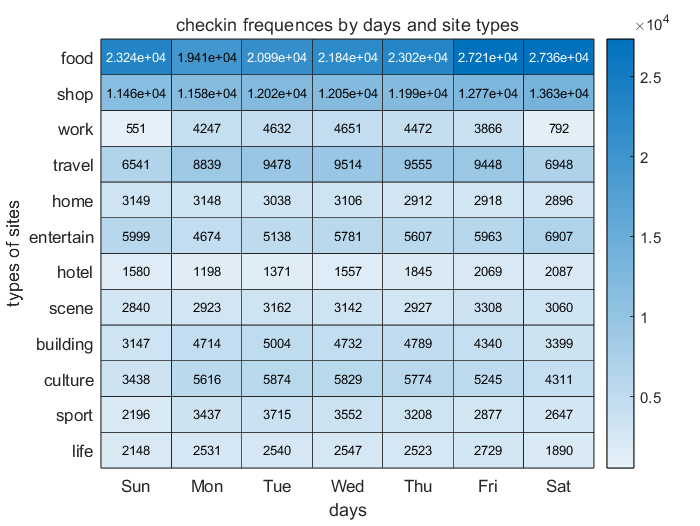
\includegraphics[scale=0.6]{day_sitetype_l.png}
			\caption{签到数关于地点类型与一周各日的分布}
			\label{day_ven}
		\end{figure}
		\begin{figure}[h]
			\centering
			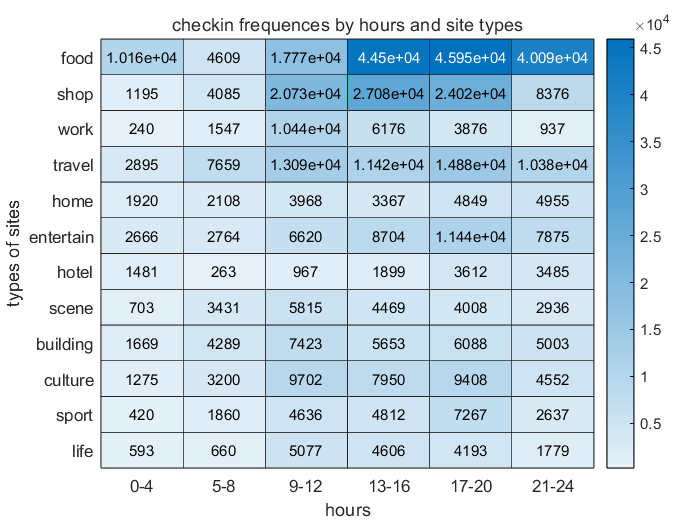
\includegraphics[scale=0.6]{hour_sitetype_l.png}
			\caption{签到数关于地点类型与小时段的分布}
			\label{hour_ven}
		\end{figure}
		
		图\ref{day_ven} 可见 food 餐饮主要集中在星期五到星期天的周末时光;shop 购买比较均匀;travel 通勤在工作日比较高,同样工作日较高的还有建筑(城市、大堂、公司、地标等)、文化教育设施(学校、图书馆、博物馆等)。
		
		图\ref{hour_ven} 可见 food 餐饮主要集中在13-20点下午直到深夜的时间;shop 购物主要集中在9-20点,应为营业时间;travel 主要通勤集中在9-12和17-20中,对应上下班早晚高峰;entertain 娱乐(公园、广场、影院、俱乐部)和 sport 运动在17-20点较高,比较符合人们的作息活动。
		
		单独香港和旧金山的地点类型-小时段签到数图如图\ref{hour_ven_hs}(调用 venhd 函数输出关联数量矩阵),可以发现除了前述的特点外城市之间大致类似。
		\begin{figure}[H]
			\centering
			\subfigure[hk]{
				\label{hour_ven_h}
				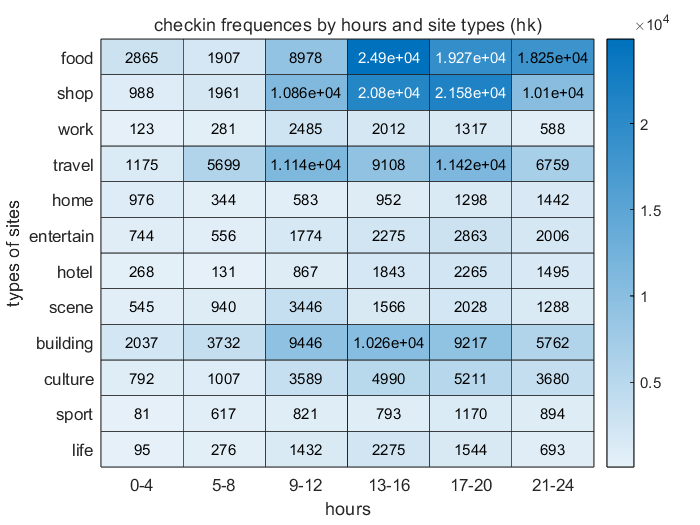
\includegraphics[scale=0.3]{hour_sitetype_l_hk.png}
			}\subfigure[sfo]{
				\label{hour_ven_s}
				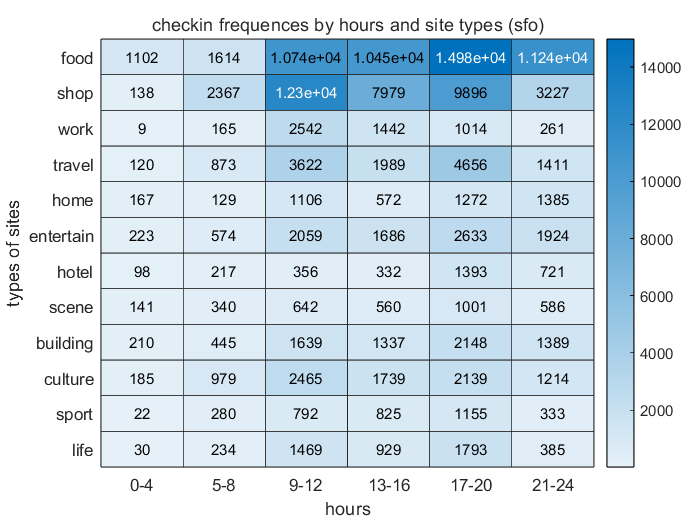
\includegraphics[scale=0.3]{hour_sitetype_l_sfo.png}
			}
			\caption{hk、sfo 签到数关于地点类型与小时段的分布}
			\label{hour_ven_hs}
		\end{figure}
		
		通过对签到热度时间性的分析可以助力商家更好的把控客流和宣传活动,在消费者活跃的时段加大投入。
		
		\subsection{签到地理热度与时空间距}
		根据nyc、hk、sfo三座城市签到地点的经纬度数据制作地理热度图得到
		
		\begin{figure}[H]
			\centering
			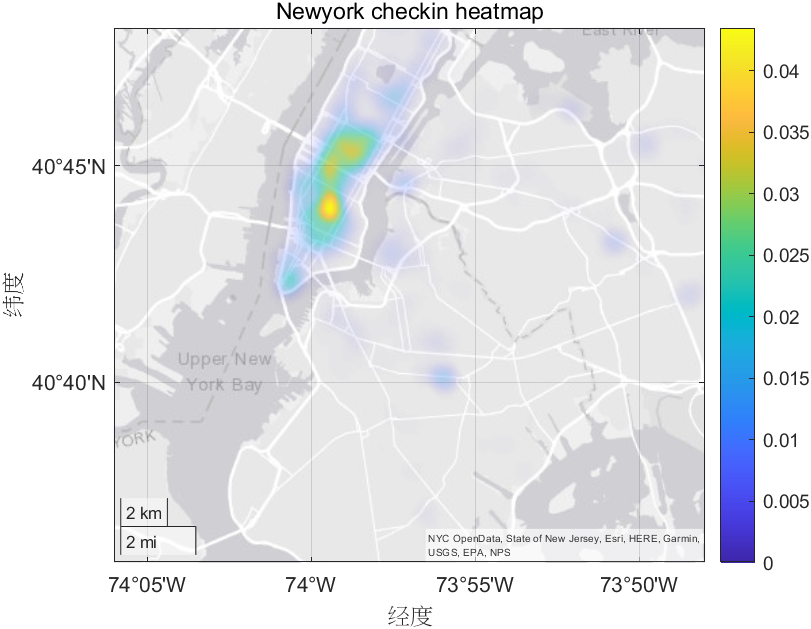
\includegraphics[scale=0.6]{geodense_nyc.png}
			\caption{纽约签到地理热度分布}
			\label{geo_n}
		\end{figure}
		\begin{figure}[H]
			\centering
			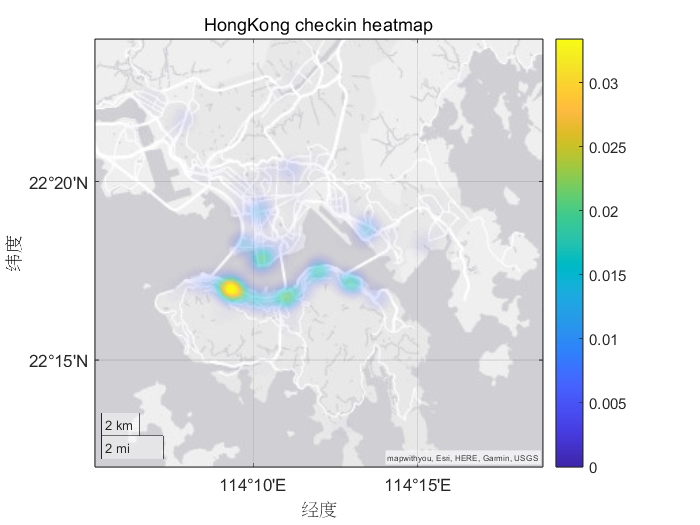
\includegraphics[scale=0.5]{geodense_hk.png}
			\caption{香港签到地理热度分布}
			\label{geo_h}
		\end{figure}
		\begin{figure}[H]
			\centering
			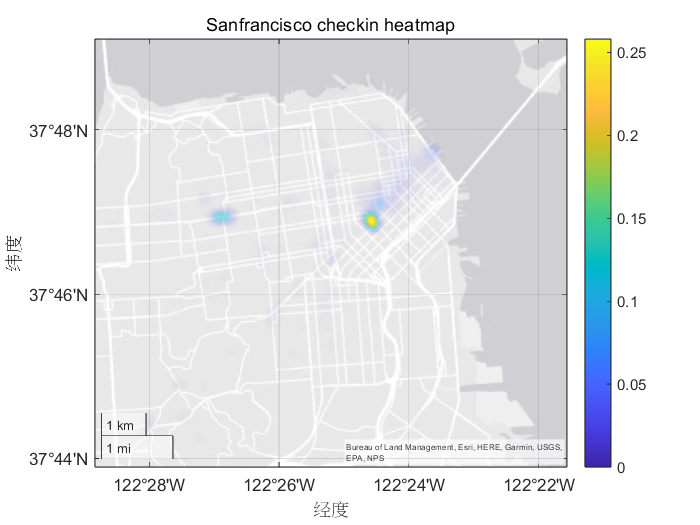
\includegraphics[scale=0.5]{geodense_sfo.png}
			\caption{旧金山签到地理热度分布}
			\label{geo_s}
		\end{figure}
		
		Swarm软件可以通过搜集签到热度的分布(比此图更加精细)来掌握客流密度的时空规律,为商家选址、投放广告提供信息,调整服务目标。
		
		接着调用 idval 函数,按照 profile 中给出的用户id搜索 checkin 数据表得到所有各个用户的签到集(删去约三百余个不匹配的无效用户),作差并统计逐次打卡的时间和空间间隔(单位:km、h),得到
		
		\begin{figure}[H]
			\centering
			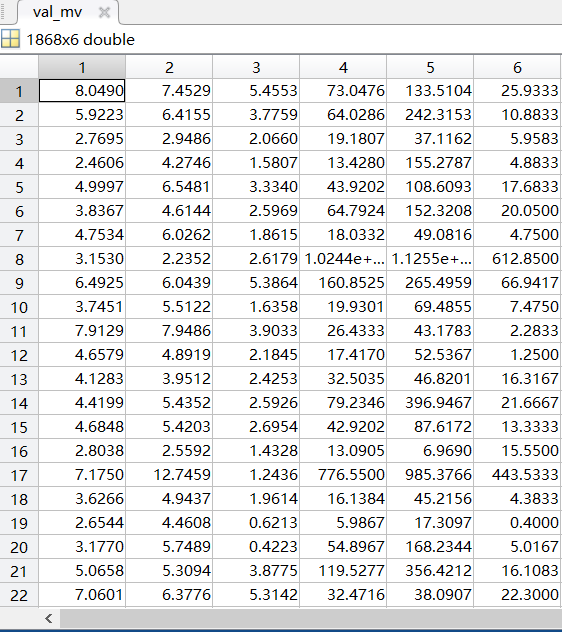
\includegraphics[scale=0.4]{val_mv.png}
			\caption{各用户空间距离的均值、标准差、中值和时间距离的均值、标准差、中值节选}
			\label{val_mv}
		\end{figure}
		\begin{figure}[H]
			\centering
			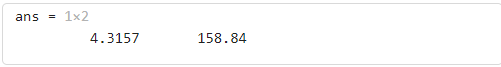
\includegraphics{val_mean.png}
			\caption{用户平均打卡间距(km、h)}
			\label{val_mean}
		\end{figure}
	
		可见用户两次签到之间距离平均为4km,时间相差将近七天(一星期)。不过不宜过度解读,可以看到尽管用户打卡距离均值在2-8km左右波动,但各用户自己各次打卡间距的方差非常大,时而登时而不登。
	
	\section{用户数据分析}
		\subsection{用户特征数分布}
		用户特征三数指 profile 表中给出的各用户签到发布数目、照片发布数目、好友数目,可能表现了用户的喜好和内外向、社交活跃度(见后可知其实几乎没有显著的关联)。对 profile 表后三列分别使用 histogram 统计得到(区分男女,未纳入性别为"none"的少量用户)
		
		\begin{figure}[H]
			\centering
			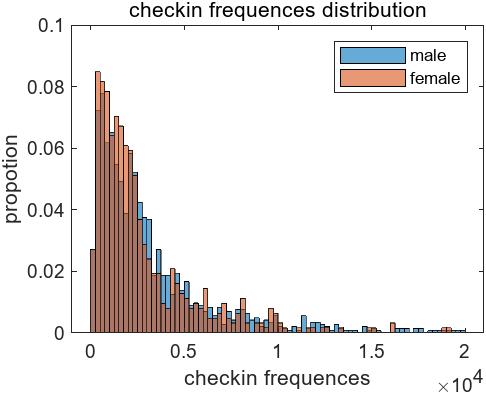
\includegraphics{checkinDis_male&female.png}
			\caption{男女用户签到数分布}
			\label{cd_mf}
		\end{figure}
		\begin{figure}[H]
			\centering
			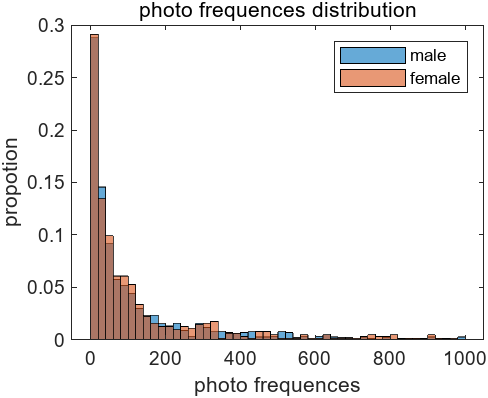
\includegraphics{photoDis_male&female.png}
			\caption{男女用户照片数分布}
			\label{pd_mf}
		\end{figure}
		\begin{figure}[H]
			\centering
			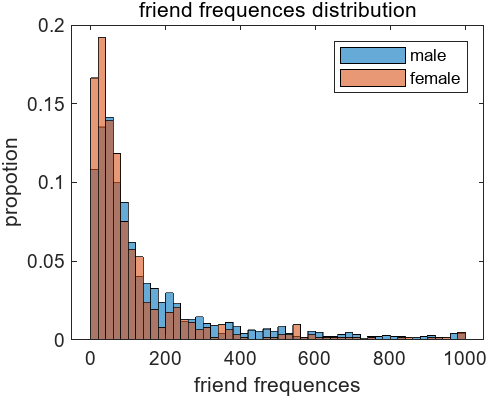
\includegraphics{friendDis_male&female.png}
			\caption{男女用户好友数分布}
			\label{fd_mf}
		\end{figure}
	
		可见签到数的峰值位于250-500区间,照片数峰值位于0-20区间,好友数峰值位于20-40区间。除去基本的签到数和一些好友,绝大多数人并没有受到继续签到或社交活跃的激励,随着数量增多其用户数迅速下降。有趣的是,反而三数均为男用户分布往右移一些(偏多一些)。三数的均值分别为(六个ans按顺序为 checkin male/female、photo male/female、friend male/female)
		
		\begin{figure}[H]
			\centering
			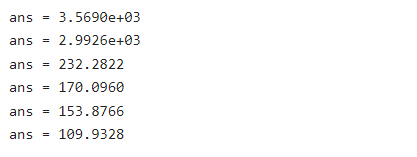
\includegraphics[scale=0.8]{cpf_mean.png}
			\caption{男女用户特征数均值}
			\label{cpf_mean}
		\end{figure}
		
		远远高于中位值和峰值,是由于部分特别大的离群点的存在。三数的极值分别为(三个ans按顺序为nyc、hk、sfo三座城市的用户的checkin、photo、friend)
		
		\begin{figure}[H]
			\centering
			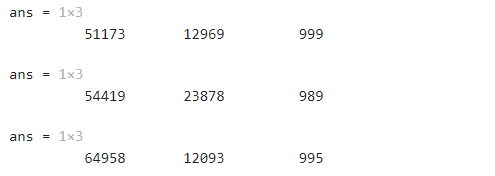
\includegraphics[scale=0.7]{nhs_max.png}
			\caption{三城用户特征数极值}
			\label{nhs_max}
		\end{figure}
		
		再以同样方式对三座城市分别统计并作图比较:
		
		\begin{figure}[H]
			\centering
			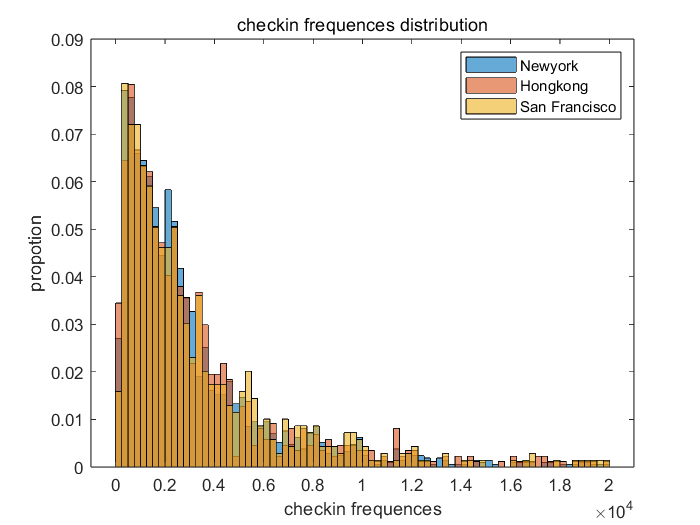
\includegraphics[scale=0.4]{checkinDis_all_nhs.png}
			\caption{三城用户签到数分布}
			\label{cd_nhs}
		\end{figure}
		\begin{figure}[H]
			\centering
			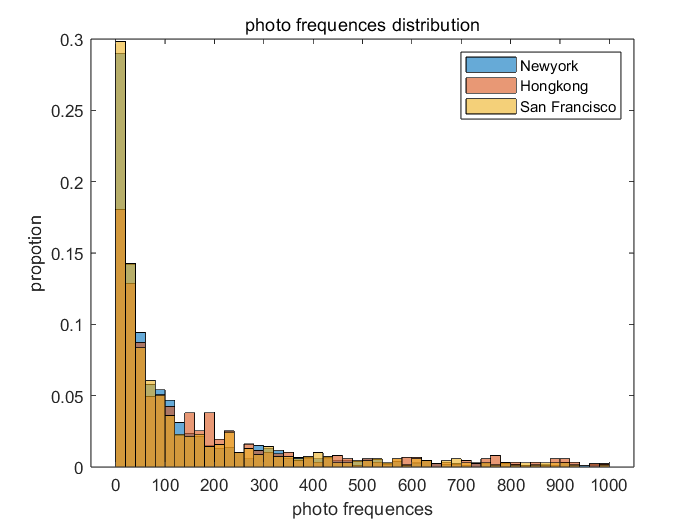
\includegraphics[scale=0.4]{photoDis_all_nhs.png}
			\caption{三城用户照片数分布}
			\label{pd_nhs}
		\end{figure}
		\begin{figure}[H]
			\centering
			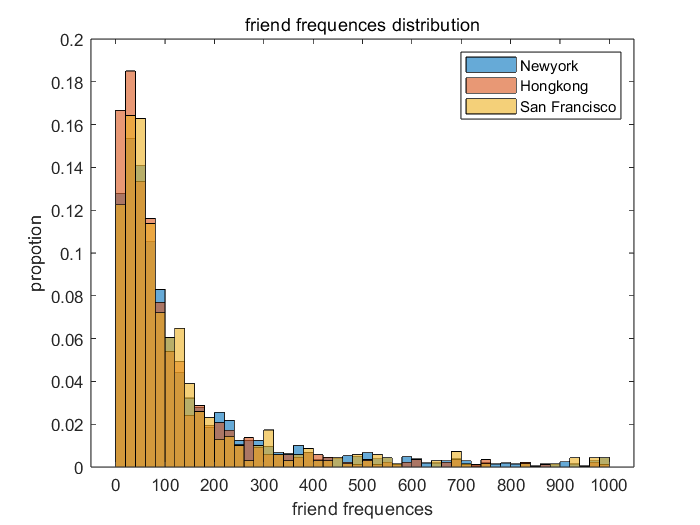
\includegraphics[scale=0.4]{friendDis_all_nhs.png}
			\caption{三城用户好友数分布)}
			\label{fd_nhs}
		\end{figure}
	
		可以发现,纽约和旧金山总的而言拥有更多的签到数和好友数;香港用户好友数大概率更少,照片数相对较多,说明其社交圈子相对封闭和稳定,这可能与中西方文化氛围有关。
		
		另外,不难看出所有特征数都是明显的偏态分布,且对其取对数后如图\ref{logdis} 所示,具有较完善细致的正态形状(除左侧略厚尾),故采用 fitdist 对数正态分布对其进行近似。
		
		\begin{figure}[H]
			\centering
			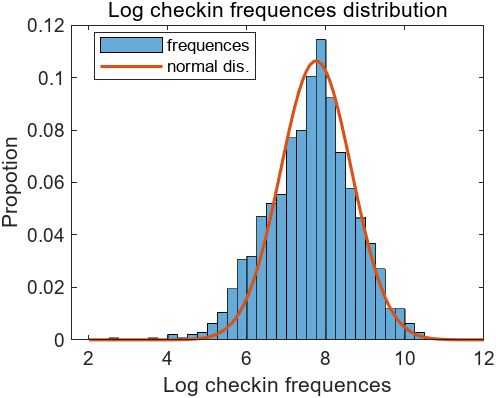
\includegraphics{logcheckinDis.png}
			\caption{用户签到数自然对数分布}
			\label{logdis}
		\end{figure}
		\begin{figure}[H]
			\centering
			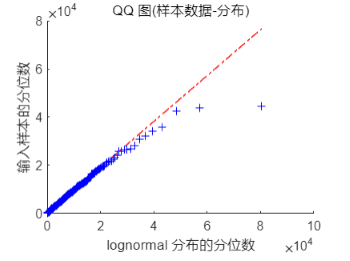
\includegraphics{qq.png}
			\caption{对数正态拟合及QQ图检验}
			\label{qq}
		\end{figure}
		
		从QQ图(图\ref{qq})亦可发现,除去右端个别偏离较大的点以外,分位数较小处基本可以完全符合对数正态分布。图\ref{chi2} 展示的结果为 chi2gof 卡方检验,P值达到了0.61,非常显著。
		
		\begin{figure}[H]
			\centering
			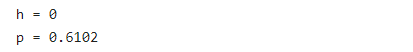
\includegraphics{chi2.png}
			\caption{卡方检验结果,接受0假设}
			\label{chi2}
		\end{figure}
		
		\subsection{用户特征数与签到地点类型、小时段的相关性}
		导入用户的签到数、照片数、好友数和其签到的小时段频数与地点类型频数,对所有这些用户指标做相关分析。下图均采用了 Pearson 相关系数,样本为nyc本地加外地用户集(经检验不同城市几乎一致),pval 为零假设的P值。
		
		\begin{figure}[H]
			\centering
			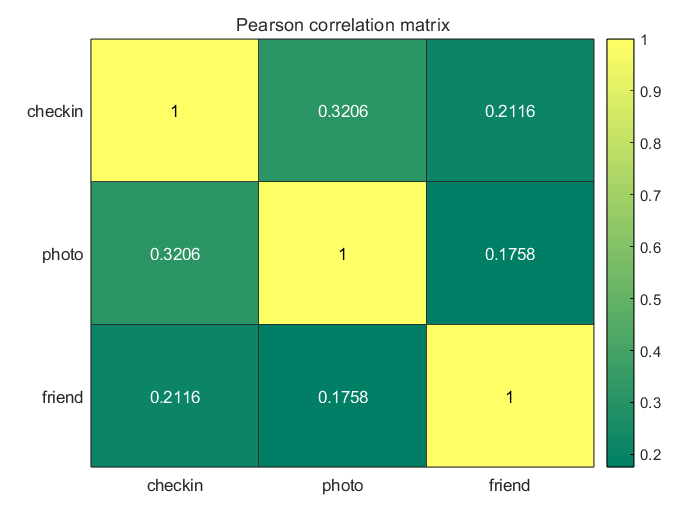
\includegraphics[scale=0.5]{cor_cpf.png}
			\caption{用户特征数相关系数矩阵}
			\label{cor_cpf}
		\end{figure}
		\begin{figure}[H]
			\centering
			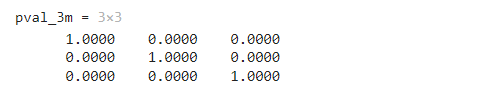
\includegraphics[scale=0.5]{pval_cpf.png}
			\caption{用户特征数相关阵检验P值}
			\label{pval_cpf}
		\end{figure}
	
		\begin{figure}[H]
			\centering
			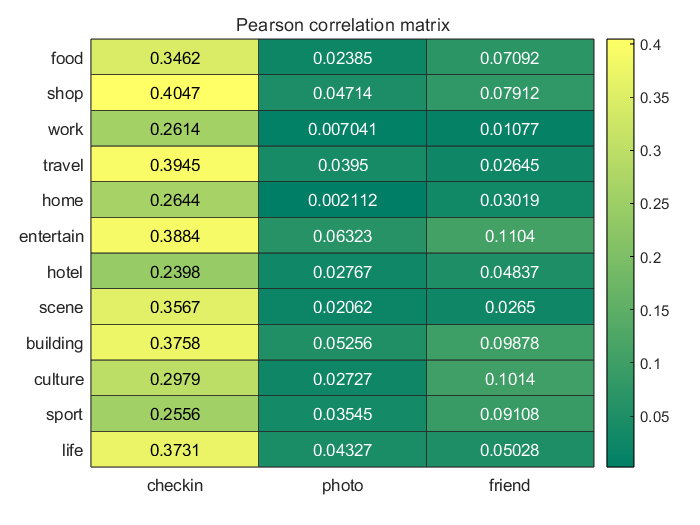
\includegraphics[scale=0.6]{cor_cpf_sitetype.png}
			\caption{用户特征数与地点类型签到数相关系数矩阵}
			\label{cor_cpf_ven}
		\end{figure}
		\begin{figure}[H]
			\centering
			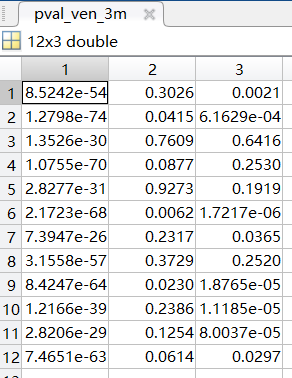
\includegraphics[scale=0.8]{pval_ven.png}
			\caption{用户特征数与地点类型签到数相关阵检验P值}
			\label{pval_ven}
		\end{figure}
	
		\begin{figure}[H]
			\centering
			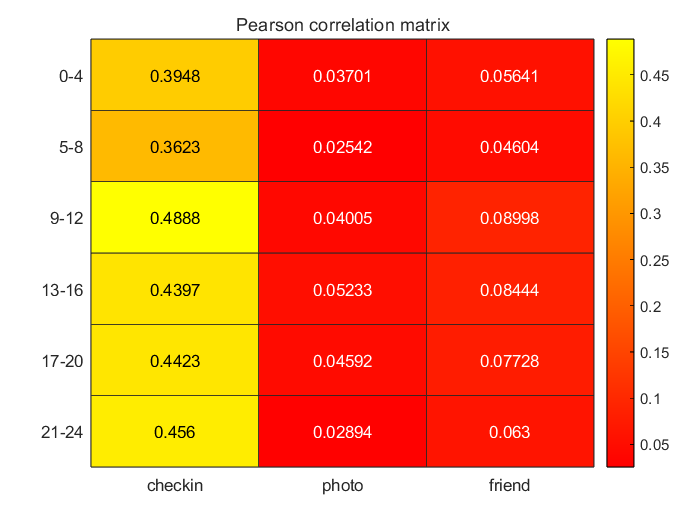
\includegraphics[scale=0.6]{cor_cpf_hour.png}
			\caption{用户特征数与小时段签到数相关系数矩阵}
			\label{cor_cpf_hour}
		\end{figure}
		\begin{figure}[H]
			\centering
			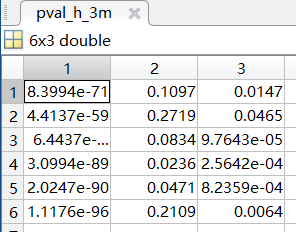
\includegraphics[scale=0.8]{pval_hour.png}
			\caption{用户特征数与小时段签到数相关阵检验P值}
			\label{pval_hour}
		\end{figure}
		
		观察P值阵可以发现,尽管相关性由于多样化的个体差异都没有很高,但许多仍然在统计学意义上具有显著的(偶然因素不足以解释的)正相关关系。其中,签到数基本可以肯定与各地点、各时段频数的关系;照片数与娱乐、生活、建筑,及12-16有显著关系(看来爱这些活动的人比较爱发照片);好友数可能是一个更优的指标,其明显的关系更多,饮食、购物、娱乐、文化、运动都非常显著且几乎全部时段都有很明显的正相关。
		
		\subsection{用户签到特征因子分析}
		首先尝试将所有指标(变量)包括十二个地点类型、六个小时段签到数、用户特征三数合在一起进行因子分析,在三个因子情况下(默认使用 varimax,在主成分基础上正交旋转以使各因子载荷方差达到最大)得到剩余方差(特殊因子方差)为
		
		\begin{figure}[H]
			\centering
			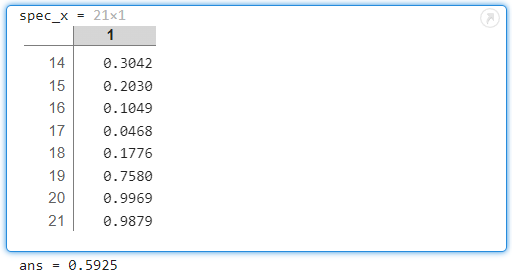
\includegraphics{fac_x.png}
			\caption{全部变量在三因子下的剩余方差}
			\label{fac_x}
		\end{figure}
		
		共同度仅0.59。观察发现最后三个变量(即用户三数)几乎未被解释(剩余方差接近1),难以匹配地点类型和小时段变量,即使提高一定的因子数目仍然无法缓解。最终在根据 spec 中方差的解释度筛选出11个变量进行因子分析,分别为 \textbf{food}、\textbf{shop}、\textbf{travel}、\textbf{scene}、\textbf{building}、\textbf{culture}、\textbf{4-8}、\textbf{8-12}、\textbf{12-16}、\textbf{16-20}、\textbf{20-24}。可见起初部分类型设置的不好,无法具有明显的表征性,理应删去。
		
		由此重新进行因子分析,设置因子数目为3,得到
		
		\begin{figure}[H]
			\centering
			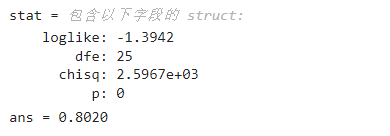
\includegraphics{fac_p.png}
			\caption{(经筛选)变量三因子分析的显著性和解释度}
			\label{fac_p}
		\end{figure}
		
		三个因子对此11个变量的解释度超过了80\%且高度显著。同时得到因子载荷阵 loading,为方便观察,将其从三个侧面作图:
		
		\begin{figure}[H]
			\centering
			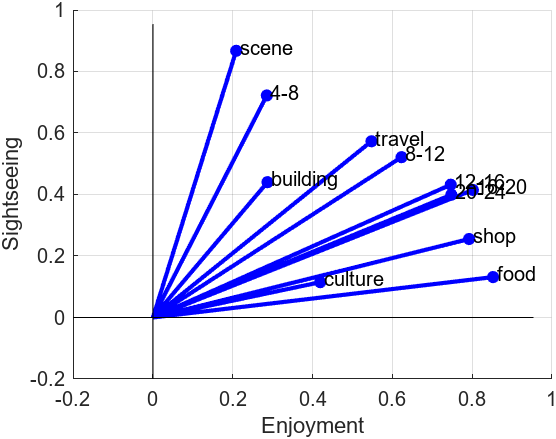
\includegraphics{fac3_s&e.png}
			\caption{各变量在因子1与因子2上的载荷}
			\label{fac_se}
		\end{figure}
		\begin{figure}[H]
			\centering
			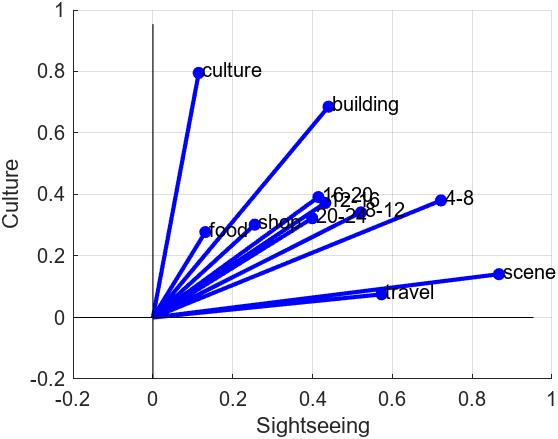
\includegraphics{fac3_s&c.png}
			\caption{各变量在因子1与因子3上的载荷}
			\label{fac_sc}
		\end{figure}
		\begin{figure}[H]
			\centering
			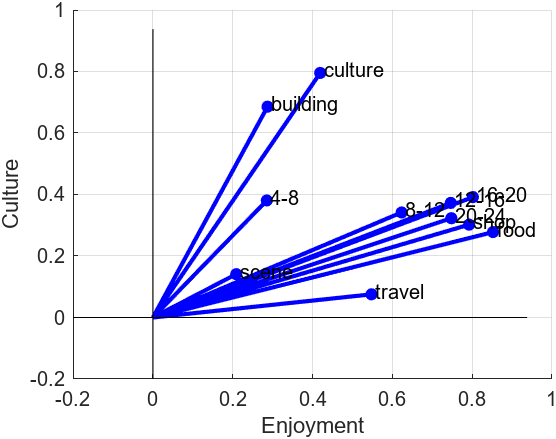
\includegraphics{fac3_c&e.png}
			\caption{各变量在因子2与因子3上的载荷}
			\label{fac_ce}
		\end{figure}
		
		根据载荷阵可以发现,不同因子有明显的不同的模式,本文将其分别命名为 \textbf{enjoyment} 玩乐因子、\textbf{sightseeing} 观光因子和 \textbf{culture} 文化因子。玩乐因子倾向于饮食购物(\textbf{food}、\textbf{shop}以及一定的\textbf{travel}),且时间集中于下午至半夜,4-8 的活动量极低;观光因子专注于户外风景(\textbf{scene},一定的\textbf{travel}和\textbf{building}),且4-8特别明显,8-12第二高(看来喜欢观光的人普遍能早起),饮食(\textbf{food})相当低(看来都不爱好研究吃);文化因子对建筑城市、教育艺术(\textbf{building}、\textbf{culture})特别出众,饮食购物一般且不热衷出行风景,时间上各个时段活动基本均匀。
		
		此外,更多因子如4个或采取 promax 方法的斜交因子模型也能达到同样好的效果(可以参看 scrap.mlx)。这里的3因子是最经济便捷且有效、有现实意义的模型。
		
		我们知道,打卡和活动的地点位置是个人及其重要的信息,正如FourSquare官网所展示的——``Harness the power of location data”,Swarm的商业价值是非常巨大的。这里只是较粗略的划分了十几个地点种类和时段,如果进一步考察各个场所,给予更详细的区分和记录,再进行聚类,一定能够制造更加精准和精细化(更多因子)的用户画像,从而为商业决策提供支持。
		
		\subsection{用户签到特征聚类}
		从另一角度看,也可以根据全部用户数据集(删去极个别 checkin.csv 和 profile.csv 无法对应的用户)计算各个变量之间的距离(相关性)来探讨。本文使用 pdist "correlation"($1-r$)表征变量距离,类平均法表征类间距进行层次聚类(dendrogram函数)得到
		
		\begin{figure}[H]
			\centering
			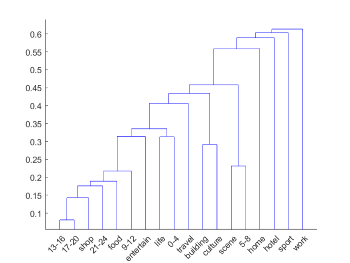
\includegraphics[scale=0.6]{group.png}
			\caption{各变量聚类谱系图}
			\label{group}
		\end{figure}
		
		从图\ref{group} 可以一览变量的亲近程度。同样的方式还可以对数据库中的众多用户进行样本聚类,既可以使用原始的各个变量,也可以使用 F(3.3节)即因子得分(默认为巴特莱特因子得分) ,得到千余个用户的聚类情况,这对软件和商家精准目标客户群体、管理应用账号和针对性服务推送有很大的意义,但在这里没有展示大量详细数值结果的意义。
		
		\subsection{本地与外地用户判别}
		本文简单的利用原本地和外地用户数据进行一次训练,采用二次判别(经检验,马氏距离效果不佳),错判率使用回判的方式(逐一对训练集中样本进行判别,估计的一般稍偏低)。
		
		\begin{figure}[H]
			\centering
			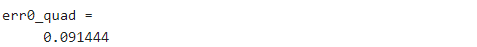
\includegraphics{err_quad.png}
			\caption{用户样本(使用21个原始变量)回判错误率}
			\label{err}
		\end{figure}
		\begin{figure}[H]
			\centering
			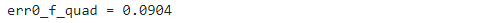
\includegraphics{err_f.png}
			\caption{用户样本(使用3个公因子)回判错误率}
			\label{err_f}
		\end{figure}
		
		结果来看能够低达9\%,算是不错的判别效果。由于判别分析已由函数一并封装,但从原理可知,通过获取一个用户的一些表征变量(如各类型地点访问数、好友数等),计算他与两样本群体(本地与外地)的距离即可方便有效的给出预测。
		
	\section{小结}
	略
	
\end{document}